%
%  untitled
%
%  Created by Drew Conway on 2010-05-24.
% 
%
\documentclass[xcolor=dvipsnames, 9pt]{beamer}

\newenvironment{code}{\begin{semiverbatim} \begin{footnotesize}}
{\end{footnotesize}\end{semiverbatim}}

\usepackage{graphicx}
\usepackage{amssymb}
\usepackage{amsfonts}
\usepackage{amsmath}
\usepackage{hyperref}
\usepackage{natbib}
\usepackage{color}
\usepackage{pdfsync}
\usepackage{chancery}
\usepackage{movie15}
\usepackage{pgfpages}
\usepackage{fancyvrb}
\usepackage{colortbl}

% \definecolor{white}{rgb}{255,255,255}
% \definecolor{darkred}{rgb}{0.5,0,0}
% \definecolor{darkgreen}{rgb}{0,0.5,0}
% \definecolor{lightblue}{rgb}{0,0,0.7}

% \hypersetup{colorlinks,
%   linkcolor=white,
%   filecolor=darkred,
%   urlcolor=lightblue,
%   citecolor=darkblue}

\usepackage{beamerthemesplit}
\usetheme{Copenhagen}
\usecolortheme[named=Violet]{structure} 
\setbeamertemplate{navigation symbols}{}
\setbeamertemplate{itemize items}[triangle]
\setbeamertemplate{enumerate items}[default]
%\setbeameroption{show notes on second screen}
% \logo{
\includegraphics[width = 2cm]{../images/logos/500px-NYU_logo.png}}

\newcommand{\R}{\mathbb{R}}
\renewcommand{\d}{\mathsf{d}}
\newcommand{\dd}{\partial}
\newcommand{\E}{\mathsf{E}}
\newcommand{\bb}{\mathbf}

\title{Module II - Why do SNA in NetworkX}
\author{Drew Conway --- Department of Politics}
\institute{
\includegraphics[width = 4cm]{../images/logos/500px-NYU_logo.png}}
\date{June 29, 2010}

\begin{document} 

\begin{frame}[plain]
  \titlepage  
\end{frame}

\begin{frame}
	\frametitle{Agenda for Module II}
	Speed and scalability
	\begin{itemize}
	   \item Why speed and scalability matter
	   \item NetworkX is designed for large data sets
	   \item Comparing NetworkX to other SNA tools
	\end{itemize}
	\uncover<2->{How NetworkX complements Python's scientific computing suite
	\begin{itemize}
	   \item SciPy/NumPy
	   \item Matplotlib
	   \item and others...
	\end{itemize}
	}
	\uncover<3->{Getting data in and out of NetworkX
	\begin{itemize}
	   \item I/O basics
	   \item Pulling non-local data
	   \begin{itemize}
	       \item Directly from the web
	       \item External databases
	   \end{itemize}
	\end{itemize}
	}
\end{frame}

\section{Speed and scalability} % (fold)
\label{sec:speed_and_scalability}

\begin{frame}[fragile]
    \frametitle{Why should we worry about scalability?}
    The size of networks being studying has increased rapidly over the years...
    \begin{center}
        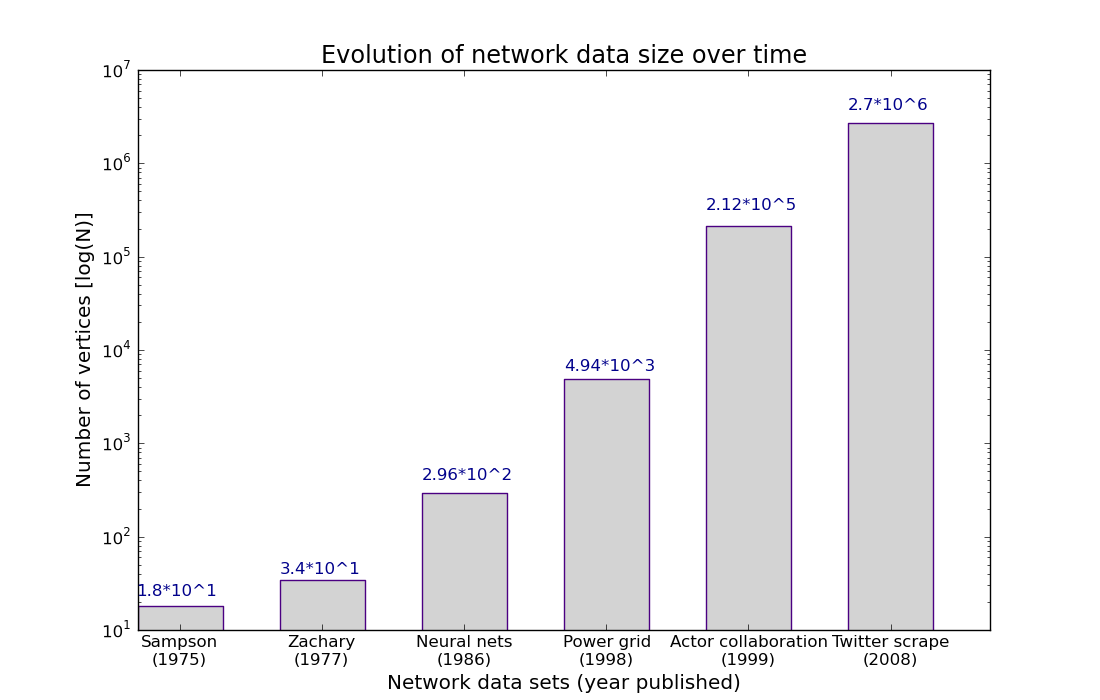
\includegraphics[scale=.37]{../images/figures/net_size_evo.png}
    \end{center}
    \uncover<3->{\alert{As network data becomes more readily available this trend will continue!}}
\end{frame}

\begin{frame}[fragile]
    \frametitle{How network size affects tools}
    While the data continues to scale up, many tools have not kept pace
    \begin{itemize}
        \item 
    \end{itemize}
\end{frame}


% section speed_and_scalability (end)

\end{document}
